\section{Generalization \& Overfitting}
\begin{frame}{Algorithm Problem: Generalization}
    \centering
    \begin{columns}[T]
        % --- Column 1: Simple fit ---
        \begin{column}{0.32\textwidth}
            \centering
            \textbf{\small Model A}\\[0.3em]
            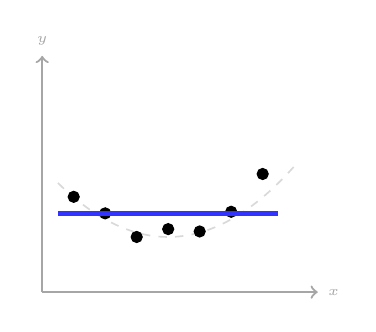
\begin{tikzpicture}[scale=1.0]
                % Axes
                \draw[->, thick, gray!70] (0,0) -- (3.5,0) node[right] {\tiny $x$};
                \draw[->, thick, gray!70] (0,0) -- (0,3) node[above] {\tiny $y$};
                % True curve (hidden to the model, just our reference)
                \draw[gray!30, dashed, line width=0.6pt, domain=0.2:3.2, samples=50] 
                    plot (\x, {0.35*(\x-1.6)^2 + 0.7});
                % Training data points
                \foreach \x/\y in {0.4/1.21, 0.8/1.0, 1.2/0.70, 1.6/0.80, 2.0/0.77, 2.4/1.02, 2.8/1.5}
                    \filldraw[black] (\x,\y) circle (2pt);
                % Simple model: flat line
                \draw[blue!80, line width=2pt] (0.2,1.0) -- (3.0,1.0);
            \end{tikzpicture}
            \vspace{0.3em}
            {\footnotesize Train MSE $\approx 0.20$}
        \end{column}
        
        % --- Column 2: Reasonable fit ---
        \begin{column}{0.32\textwidth}
            \centering
            \textbf{\small Model B}\\[0.3em]
            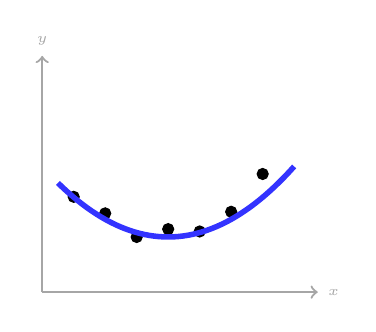
\begin{tikzpicture}[scale=1.0]
                % Axes
                \draw[->, thick, gray!70] (0,0) -- (3.5,0) node[right] {\tiny $x$};
                \draw[->, thick, gray!70] (0,0) -- (0,3) node[above] {\tiny $y$};
                % Training data points
                \foreach \x/\y in {0.4/1.21, 0.8/1.0, 1.2/0.70, 1.6/0.80, 2.0/0.77, 2.4/1.02, 2.8/1.5}
                    \filldraw[black] (\x,\y) circle (2pt);
                % Smooth curve through the trend
                \draw[blue!80, line width=2pt, domain=0.2:3.2, samples=50] 
                    plot (\x, {0.35*(\x-1.6)^2 + 0.7});
            \end{tikzpicture}
            \vspace{0.3em}
            {\footnotesize Train MSE $\approx 0.06$}
        \end{column}
        
        % --- Column 3: Very wiggly fit ---
        \begin{column}{0.32\textwidth}
            \centering
            \textbf{\small Model C}\\[0.3em]
            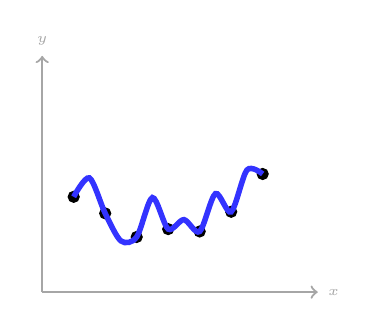
\begin{tikzpicture}[scale=1.0]
                % Axes
                \draw[->, thick, gray!70] (0,0) -- (3.5,0) node[right] {\tiny $x$};
                \draw[->, thick, gray!70] (0,0) -- (0,3) node[above] {\tiny $y$};
                % Training data points
                \foreach \x/\y in {0.4/1.21, 0.8/1.0, 1.2/0.70, 1.6/0.80, 2.0/0.77, 2.4/1.02, 2.8/1.5}
                    \filldraw[black] (\x,\y) circle (2pt);
                % Wiggly curve going exactly through points
                \draw[blue!80, line width=2pt, smooth] 
                    plot coordinates {
                        (0.4,1.21) (0.6,1.45) (0.8,1.0) (1.0,0.65) 
                        (1.2,0.70) (1.4,1.2) (1.6,0.8) (1.8,0.92) 
                        (2.0,0.77) (2.2,1.25) (2.4,1.02) (2.6,1.55) (2.8,1.5)
                    };
            \end{tikzpicture}
            \vspace{0.3em}
            {\footnotesize Train MSE $\approx 0.00$}
        \end{column}
    \end{columns}
    
    \vspace{0.6em}
    \centering
    \small
    All three models see the same training points but fit them in very different ways.  
    Which one should we pick?
\end{frame}

\begin{frame}{What Do We Really Want?}
    \begin{itemize}
        \item We care about how the model behaves on \textbf{new unseen data}, not only on the points it has already seen
        \item Imagine we now collect a few fresh samples from the same process
    \end{itemize}
    
    \vspace{0.6em}
    \centering
    \begin{columns}[T]
        % --- Column 1: Model A with new points ---
        \begin{column}{0.32\textwidth}
            \centering
            \textbf{\small Model A}\\[0.3em]
            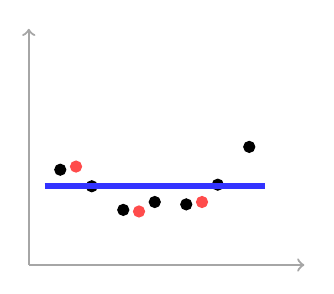
\begin{tikzpicture}[scale=1.0]
                % Axes
                \draw[->, thick, gray!70] (0,0) -- (3.5,0);
                \draw[->, thick, gray!70] (0,0) -- (0,3);
                % Training data
                \foreach \x/\y in {0.4/1.21, 0.8/1.0, 1.2/0.70, 1.6/0.80, 2.0/0.77, 2.4/1.02, 2.8/1.5}
                    \filldraw[black] (\x,\y) circle (2pt);
                % New data points (e.g. test)
                \foreach \x/\y in {0.6/1.25, 1.4/0.68, 2.2/0.8}
                    \filldraw[red!70] (\x,\y) circle (2pt);
                % Simple model
                \draw[blue!80, line width=2pt] (0.2,1.0) -- (3.0,1.0);
            \end{tikzpicture}
        \end{column}
        
        % --- Column 2: Model B with new points ---
        \begin{column}{0.32\textwidth}
            \centering
            \textbf{\small Model B}\\[0.3em]
            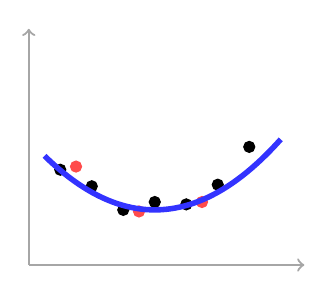
\begin{tikzpicture}[scale=1.0]
                % Axes
                \draw[->, thick, gray!70] (0,0) -- (3.5,0);
                \draw[->, thick, gray!70] (0,0) -- (0,3);
                % Training data
                \foreach \x/\y in {0.4/1.21, 0.8/1.0, 1.2/0.70, 1.6/0.80, 2.0/0.77, 2.4/1.02, 2.8/1.5}
                    \filldraw[black] (\x,\y) circle (2pt);
                % New data
                \foreach \x/\y in {0.6/1.25, 1.4/0.68, 2.2/0.8}
                    \filldraw[red!70] (\x,\y) circle (2pt);
                % Smooth curve
                \draw[blue!80, line width=2pt, domain=0.2:3.2, samples=50] 
                    plot (\x, {0.35*(\x-1.6)^2 + 0.7});
            \end{tikzpicture}
        \end{column}
        
        % --- Column 3: Model C with new points ---
        \begin{column}{0.32\textwidth}
            \centering
            \textbf{\small Model C}\\[0.3em]
            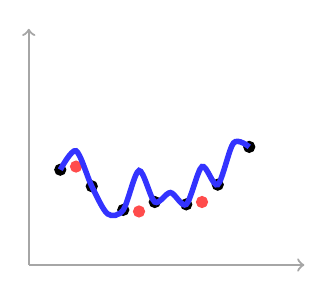
\begin{tikzpicture}[scale=1.0]
                % Axes
                \draw[->, thick, gray!70] (0,0) -- (3.5,0);
                \draw[->, thick, gray!70] (0,0) -- (0,3);
                % Training data
                \foreach \x/\y in {0.4/1.21, 0.8/1.0, 1.2/0.70, 1.6/0.80, 2.0/0.77, 2.4/1.02, 2.8/1.5}
                    \filldraw[black] (\x,\y) circle (2pt);
                % New data
                \foreach \x/\y in {0.6/1.25, 1.4/0.68, 2.2/0.8}
                    \filldraw[red!70] (\x,\y) circle (2pt);
                % Wiggly curve
                \draw[blue!80, line width=2pt, smooth] 
                    plot coordinates {
                        (0.4,1.21) (0.6,1.45) (0.8,1.0) (1.0,0.65) 
                        (1.2,0.70) (1.4,1.2) (1.6,0.8) (1.8,0.92) 
                        (2.0,0.77) (2.2,1.25) (2.4,1.02) (2.6,1.55) (2.8,1.5)
                    };
            \end{tikzpicture}
        \end{column}
    \end{columns}
    
    \vspace{0.5em}
    \small
    On these new red points, Model B stays close, while Model A and Model C miss more.  
\end{frame}

\begin{frame}{Underfit vs Good Fit vs Overfit}
    \centering
    \begin{columns}[T]
        % --- Column 1: Underfit ---
        \begin{column}{0.32\textwidth}
            \centering
            \textbf{\small Underfit}\\[0.3em]
            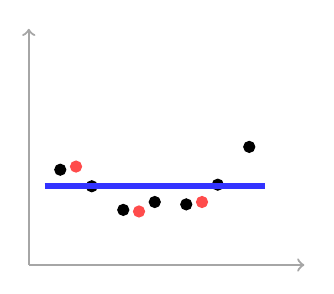
\begin{tikzpicture}[scale=1.0]
                \draw[->, thick, gray!70] (0,0) -- (3.5,0);
                \draw[->, thick, gray!70] (0,0) -- (0,3);
                % Train data
                \foreach \x/\y in {0.4/1.21, 0.8/1.0, 1.2/0.70, 1.6/0.80, 2.0/0.77, 2.4/1.02, 2.8/1.5}
                    \filldraw[black] (\x,\y) circle (2pt);
                % New data
                \foreach \x/\y in {0.6/1.25, 1.4/0.68, 2.2/0.8}
                    \filldraw[red!70] (\x,\y) circle (2pt);
                % Simple model
                \draw[blue!80, line width=2pt] (0.2,1.0) -- (3.0,1.0);
            \end{tikzpicture}
            \vspace{0.4em}
            \begin{tcolorbox}[colback=red!5, colframe=red!40, boxrule=0.5pt, arc=2mm, left=2pt, right=2pt, top=2pt, bottom=2pt]
                \centering \small \textbf{Too Simple\\(High Bias)}\\Ignores patterns
            \end{tcolorbox}
        \end{column}
        
        % --- Column 2: Good Fit ---
        \begin{column}{0.32\textwidth}
            \centering
            \textbf{\small Good Fit}\\[0.3em]
            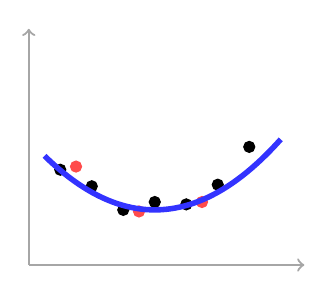
\begin{tikzpicture}[scale=1.0]
                \draw[->, thick, gray!70] (0,0) -- (3.5,0);
                \draw[->, thick, gray!70] (0,0) -- (0,3);
                % Train data
                \foreach \x/\y in {0.4/1.21, 0.8/1.0, 1.2/0.70, 1.6/0.80, 2.0/0.77, 2.4/1.02, 2.8/1.5}
                    \filldraw[black] (\x,\y) circle (2pt);
                % New data
                \foreach \x/\y in {0.6/1.25, 1.4/0.68, 2.2/0.8}
                    \filldraw[red!70] (\x,\y) circle (2pt);
                % Reasonable curve
                \draw[blue!80, line width=2pt, domain=0.2:3.2, samples=50] 
                    plot (\x, {0.35*(\x-1.6)^2 + 0.7});
            \end{tikzpicture}
            \vspace{0.4em}
            \begin{tcolorbox}[colback=green!5, colframe=black!40, boxrule=0.5pt, arc=2mm, left=2pt, right=2pt, top=2pt, bottom=2pt]
                \centering \small \textbf{Captures Structure}\\Balanced
            \end{tcolorbox}
        \end{column}
        
        % --- Column 3: Overfit ---
        \begin{column}{0.32\textwidth}
            \centering
            \textbf{\small Overfit}\\[0.3em]
            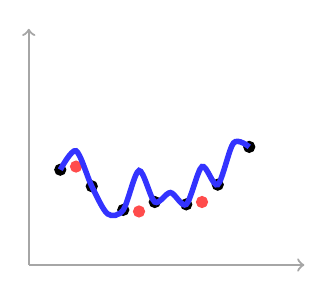
\begin{tikzpicture}[scale=1.0]
                \draw[->, thick, gray!70] (0,0) -- (3.5,0);
                \draw[->, thick, gray!70] (0,0) -- (0,3);
                % Train data
                \foreach \x/\y in {0.4/1.21, 0.8/1.0, 1.2/0.70, 1.6/0.80, 2.0/0.77, 2.4/1.02, 2.8/1.5}
                    \filldraw[black] (\x,\y) circle (2pt);
                % New data
                \foreach \x/\y in {0.6/1.25, 1.4/0.68, 2.2/0.8}
                    \filldraw[red!70] (\x,\y) circle (2pt);
                % Wiggly curve
                \draw[blue!80, line width=2pt, smooth] 
                    plot coordinates {
                        (0.4,1.21) (0.6,1.45) (0.8,1.0) (1.0,0.65) 
                        (1.2,0.70) (1.4,1.2) (1.6,0.8) (1.8,0.92) 
                        (2.0,0.77) (2.2,1.25) (2.4,1.02) (2.6,1.55) (2.8,1.5)
                    };
            \end{tikzpicture}
            \vspace{0.4em}
            \begin{tcolorbox}[colback=red!5, colframe=red!40, boxrule=0.5pt, arc=2mm, left=2pt, right=2pt, top=2pt, bottom=2pt]
                \centering \small \textbf{Too Complex\\(High Variance)}\\Memorizes noise
            \end{tcolorbox}
        \end{column}
    \end{columns}
\end{frame}

\begin{frame}{Underfit vs Good Fit vs Overfit}
    \begin{itemize}
        \item \textbf{Underfitting}
        \begin{itemize}
            \item Model is too simple for the true pattern
            \item It cannot reach low error even with a lot of data
        \end{itemize}
        \item \textbf{Overfitting}
        \begin{itemize}
            \item Model is too flexible and learns noise
            \item It fits training points very well but is unstable on new points
        \end{itemize}
        \item \textbf{Good fit}
        \begin{itemize}
            \item Model has just enough flexibility to capture useful structure
            \item It behaves similarly on seen and unseen data
        \end{itemize}
    \end{itemize}
\end{frame}

\begin{frame}{What is Generalization?}

    \begin{block}{Definition}
        Generalization is the ability of a model to perform well on data it has \textbf{never seen before}.
    \end{block}
    
    \vspace{1em}
    
    \textbf{High Training Accuracy $\neq$ Learning}
    \begin{itemize}
        \item \textbf{Memorization (Capacity):} Modern models are powerful enough to memorize the entire training set, acting like a "lookup table" rather than a learner.
        \item \textbf{Shortcuts (Laziness):} If a simple noise pattern correlates with the target, the model will learn that instead of the complex true signal.
    \end{itemize}

\end{frame}


\begin{frame}{Examples:}
    \centering
    \small    
    \begin{table}[]
        \centering
        \renewcommand{\arraystretch}{1.4} 
        \begin{tabular}{l p{4.0cm} p{4.5cm}}
            \hline
            \textbf{Domain} & \textbf{Intended Pattern} & \textbf{Reality} \\ \hline
            \textbf{Vision} & Recognizes animal features (ears, snout). & Learns that \textbf{snow background} = Wolf. \\ 
            \textbf{Tabular} & Evaluates financial history (income, debt). & Learns that \textbf{Application Font/ID} = High Risk. \\ 
            \textbf{NLP} & Analyzes sentence semantics and sentiment. & Memorizes specific \textbf{names} (e.g., "Ali"). \\ 
            \textbf{RL} & Learns strategy to win the game/level. & Finds a \textbf{glitch} or loops indefinitely to farm points. \\ \hline
        \end{tabular}
    \end{table}
\end{frame}


\begin{frame}{Addressing Overfitting}
    \centering
    \large \textit{Since we cannot trust the training error, we need a systematic approach to validate our models.}
    
    \vspace{0.8cm}
    
    \begin{columns}[T]
        \begin{column}{0.3\textwidth}
            \begin{block}{\centering1. Detect:}
                \centering
                \textbf{Splitting Data}\\
                (Holdout, K-Fold)
            \end{block}
        \end{column}
        \begin{column}{0.3\textwidth}
            \begin{block}{\centering2. Measure:}
                \centering
                \textbf{Metrics}\\
                (Accuracy, MSE, F1, AUC)
            \end{block}
        \end{column}
        \begin{column}{0.3\textwidth}
            \begin{block}{\centering3. Mitigate:}
                \centering
                \textbf{Strategies}\\
                (Regularization, More Data, Better Features)
            \end{block}
        \end{column}
    \end{columns}
\end{frame}

\subsection{Data Splitting}

\begin{frame}{Addressing Overfitting}
    \centering
    \large \textit{Since we cannot trust the training error, we need a systematic approach to validate our models.}
    
    \vspace{0.8cm}
    
    \begin{columns}[T]
        \begin{column}{0.3\textwidth}
            \begin{block}{\centering1. Detect:}
                \centering
                \textbf{Splitting Data}\\
                (Holdout, K-Fold)
            \end{block}
        \end{column}
        \begin{column}{0.3\textwidth}
            \begin{block}{\centering2. Measure:}
                \centering
                \textbf{Metrics}\\
                (Accuracy, MSE, F1, AUC)
            \end{block}
        \end{column}
        \begin{column}{0.3\textwidth}
            \begin{block}{\centering3. Mitigate:}
                \centering
                \textbf{Strategies}\\
                (Regularization, More Data, Better Features)
            \end{block}
        \end{column}
    \end{columns}
    
    \vspace{0.5cm}
    \centering
    \small $\rightarrow$ \textit{Step 1: How to simulate "unseen data" using Splits.}
\end{frame}
